%----------------------------------------------------------------------------------------
%
% LaTeX-mall för examensarbeten vid LNU
% Skapad av Marcus Wilhelmsson, Institutionen för Datavetenskap
% Fakulteten för Teknik
% Linnéuniversitetet
%
% Licens: Creative Commons BY
%
%----------------------------------------------------------------------------------------

%----------------------------------------------------------------------------------------
%	Inställningar och dokumentkonfiguration
%----------------------------------------------------------------------------------------

\documentclass[paper=a4, fontsize=11pt]{article} % A4-sida och 11 punkters fontstorlek

\usepackage[T1]{fontenc} % 8-bitarskodning som har 256 glyfer
\usepackage{times} % Typsnitt i dokumentet
\usepackage[swedish,english]{babel} % Svenskt språk, engelska för extra abstract
\usepackage[utf8]{inputenc} % För svenska tecken (UTF-8)
\usepackage{dtklogos} % Logos för t.ex. LaTeX, BibTeX, etc.
\usepackage{wallpaper} % Bakgrundsbild
\usepackage[absolute]{textpos} % Möjlighet att absolutpositionera text
\usepackage[top=2cm, bottom=2.5cm, left=3cm, right=3cm]{geometry} % Ställ in marginaler
\usepackage{appendix} % Stöd för separat hantering av bilagor

\setcounter{secnumdepth}{5} % Fem nivåer av underrubriksnumrering
\setcounter{tocdepth}{5} % Fem nivåer av underrubriksnumrering i innehållsförteckning

%----------------------------------------------------------------------------------------
%	Denna del används för att skapa boxen med författare, handledare, etc.
%----------------------------------------------------------------------------------------
\newsavebox{\mybox}
\newlength{\mydepth}
\newlength{\myheight}

\newenvironment{sidebar}%
{\begin{lrbox}{\mybox}\begin{minipage}{\textwidth}}%
{\end{minipage}\end{lrbox}%
 \settodepth{\mydepth}{\usebox{\mybox}}%
 \settoheight{\myheight}{\usebox{\mybox}}%
 \addtolength{\myheight}{\mydepth}%
 \noindent\makebox[0pt]{\hspace{-20pt}\rule[-\mydepth]{1pt}{\myheight}}%
 \usebox{\mybox}}

%----------------------------------------------------------------------------------------
%	Titel-sektion
%----------------------------------------------------------------------------------------
\newcommand\BackgroundPic{
    \put(-2,-3){
    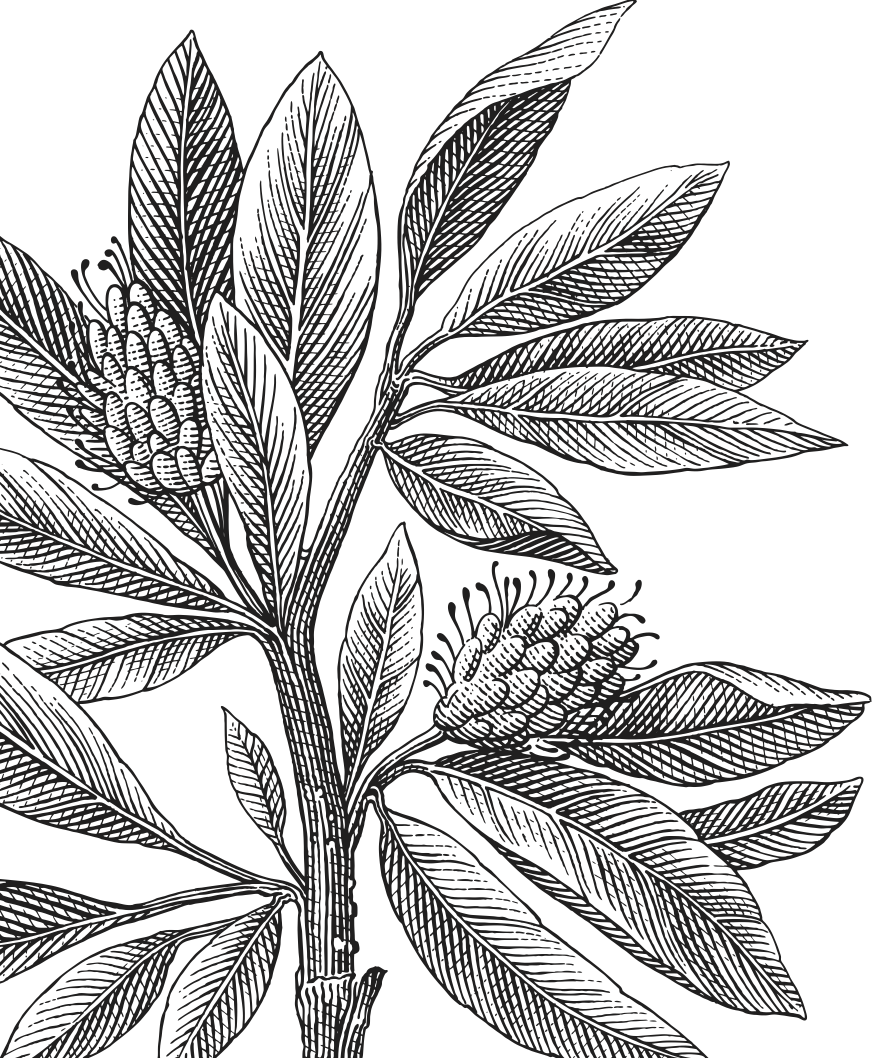
\includegraphics[keepaspectratio,scale=0.3]{img/lnu_etch.png} % Bakgrundsbild
    }
}
\newcommand\BackgroundPicLogo{
    \put(18,700){
    
\includegraphics[keepaspectratio,scale=0.10]{img/logo.png} % Logga i övre vänstra hörnet
    }
}

\title{	
\vspace{-8cm}
\begin{sidebar}
    \vspace{10cm}
    \normalfont \normalsize
    \Huge Dokumenttyp \\ % Dokumentets typ, t.ex. Examensarbete
    \vspace{-1.3cm}
\end{sidebar}
\vspace{3cm}
\begin{flushleft}
    \huge Rubrik\\ % Dokumentets rubrik
    \it \LARGE Underrubrik % Dokumentets underrubrik
\end{flushleft}
\null
\vfill
\begin{textblock}{10}(8,13)
\begin{flushright}
\begin{minipage}{0.7\textwidth}
\begin{flushleft} \large
\emph{Författare:} John \textsc{Smith}\\ % Författare
\emph{Handledare:} Dr.~Foo \textsc{Bar}\\ % Handledare
\emph{Examinator:} Dr.~Mark \textsc{Brown}\\ % Examinator
\emph{Termin:} HT2013\\ % Termin
\emph{Ämne:} Någonvetenskap\\ % Ämne
\emph{Nivå:} G2F\\ % Nivå
\emph{Kurskod:} 2DVXXX % Kurskod
\end{flushleft}
\end{minipage}
\end{flushright}
\end{textblock}
}


\date{} % Dagens datum, tomt i detta fallet. Använd \today för dagens datum.

\begin{document}
\pagenumbering{gobble}
\newgeometry{left=5cm}
\AddToShipoutPicture*{\BackgroundPic} % Lägger in backgrundsbild på första sidan
\AddToShipoutPicture*{\BackgroundPicLogo} % Lägger in LNU-logga på första sidan
\maketitle % Skriv ut titeln
\restoregeometry
\clearpage
%----------------------------------------------------------------------------------------
%	Svensk och engelsk version av abstract
%----------------------------------------------------------------------------------------
\selectlanguage{swedish}
\begin{abstract}
Lorem ipsum dolor sit amet, consectetur adipiscing elit. Pellentesque convallis arcu elit, sit amet dictum nibh semper id. Quisque non iaculis est. Mauris ornare auctor scelerisque. Sed elementum ipsum nunc, vitae placerat lacus faucibus eu. Donec vestibulum, nisi vel tristique accumsan, massa lorem rhoncus metus, quis mattis eros arcu at dui. Ut quis consequat diam. Integer et nisl id lacus sodales posuere. Integer tristique metus ac posuere consequat. Aliquam gravida mauris vitae cursus posuere. Cras mollis sem vel faucibus fermentum. Duis vitae interdum nunc. Pellentesque egestas cursus turpis, eu lobortis justo ullamcorper quis. Nullam eget dui lacinia, convallis leo imperdiet, ornare justo. Quisque mattis eleifend justo, vel interdum diam molestie sed.
\end{abstract}
\selectlanguage{english}
\begin{abstract}
The European languages are members of the same family. Their separate existence is a myth. For science, music, sport, etc, Europe uses the same vocabulary. The languages only differ in their grammar, their pronunciation and their most common words. Everyone realizes why a new common language would be desirable: one could refuse to pay expensive translators. To achieve this, it would be necessary to have uniform grammar, pronunciation and more common words. If several languages coalesce, the grammar of the resulting language is more simple and regular than that of the individual languages. The new common language will be more simple and regular than the existing European languages. It will be as simple as Occidental; in fact, it will be Occidental. To an English person, it will seem like simplified English, as a skeptical Cambridge friend of mine told me what Occidental is.The European languages are members of the same family. Their separate existence is a myth. For science, music, sport, etc, Europe uses the same vocabulary. The languages only differ in their grammar, their pronunciation and their most common words. Everyone realizes why a new common language would be desirable: one could refuse to pay expensive translators.
\end{abstract}
\selectlanguage{swedish}
%----------------------------------------------------------------------------------------
\newpage
\pagenumbering{gobble} % Stäng av sidnumrering för innehållsförteckningssidan
\tableofcontents % Innehållsförteckning
\newpage % Ny sida
\pagenumbering{arabic} % Påbörja sidnumrering på 1


%----------------------------------------------------------------------------------------
%	Rubrik 1
%----------------------------------------------------------------------------------------
\section{Rubrik 1}
Enligt \cite{small} är detta en rubrik. Enligt \cite{big} är även detta en rubrik.
%----------------------------------------------------------------------------------------
%	Underrubrik 2
%----------------------------------------------------------------------------------------
\subsection{Underrubrik 2}
Lorem ipsum dolor sit amet, consectetur adipiscing elit. Pellentesque convallis arcu elit, sit amet dictum nibh semper id. Quisque non iaculis est. Mauris ornare auctor scelerisque.
%----------------------------------------------------------------------------------------
%	Under-underrubrik 3
%----------------------------------------------------------------------------------------
\subsubsection{Underrubriksnivå 3}
Nunc molestie libero in quam commodo, id volutpat justo vehicula. Aliquam tristique leo et ullamcorper dapibus. Sed eu blandit lorem. Phasellus fermentum risus ac risus porttitor consectetur. Nunc euismod ultricies pellentesque. Quisque id dolor lorem. Nulla sollicitudin dignissim quam, a blandit sapien lobortis et.
%----------------------------------------------------------------------------------------
%	Under-under-underrubrik 4, OBS! \paragraph
%----------------------------------------------------------------------------------------
\paragraph{Underrubriksnivå 4}
Fusce suscipit faucibus dui non facilisis. Sed enim tortor, tempor nec mauris et, mollis malesuada orci. Aenean ut ullamcorper eros. Nulla vel magna at sem varius porttitor. Nam scelerisque blandit metus, ac eleifend ante rutrum nec. Fusce dignissim nisi arcu. Suspendisse iaculis odio non risus tempor consectetur. Fusce dapibus quam et nulla euismod vulputate. Vivamus quis mauris et tortor mollis ullamcorper vel luctus metus. Mauris dictum sapien ac ultricies dignissim. Morbi consequat ligula quis ipsum condimentum, ut interdum nibh auctor.
%----------------------------------------------------------------------------------------
%	Under-under-under-underrubrik 5, OBS! \subparagraph
%----------------------------------------------------------------------------------------
\subparagraph{Underrubriksnivå 5}
Curabitur consectetur nibh sit amet fringilla ornare. Aenean eu massa pharetra odio mollis accumsan. Proin accumsan condimentum pharetra. Maecenas eu nunc vitae erat mattis tincidunt vitae ut leo. Sed mauris mauris, pellentesque sed leo sit amet, molestie aliquam dui. Duis ut elit mollis, facilisis nibh non, egestas est. Fusce egestas at ligula lacinia vehicula. Maecenas bibendum consequat nisl, non suscipit enim.
%----------------------------------------------------------------------------------------
%	Referenser
%  IEEE-system med siffror för referenser
%  Ändra bibliographystyle för annat referenssystem
%
%----------------------------------------------------------------------------------------
\newpage
\bibliographystyle{ieeetr}
\bibliography{referenser}
\newpage
%----------------------------------------------------------------------------------------
%	Bilagor, hanteras i separat fil kallad appendix
%-----------------------------------------------------------------------------------------
\appendix
\section*{Bilaga 1} % Använd * för att dölja bilagan från Innehåll
Sed malesuada ligula magna, vel tempus arcu ornare vitae. Maecenas sit amet libero fermentum, sagittis nisl in, sollicitudin elit. Sed tincidunt nisi at nibh lobortis, ut dignissim lorem faucibus. Nulla tempus congue sem, ac congue eros imperdiet in. Proin at felis tincidunt, dignissim orci id, venenatis sapien. Mauris non dignissim mauris. Quisque facilisis luctus lorem a molestie. Nulla varius lorem sed magna congue, vitae fermentum orci laoreet. Fusce porta orci nec velit mollis, vitae consequat sapien mollis. In gravida luctus turpis et ullamcorper. Nunc hendrerit vel nisi non feugiat.
\begin{subappendices}
\subsection*{Bilaga 1 - Underbilaga}
Sed adipiscing ligula purus, at faucibus nisl dapibus eu. Maecenas mattis libero sit amet tellus vulputate gravida. Fusce elit tellus, vulputate at justo quis, rhoncus lacinia urna. Aliquam ornare vestibulum nunc, nec bibendum erat volutpat non. Proin ultrices sem quam. Morbi posuere, tellus at lobortis iaculis, nunc turpis ultricies diam, at dapibus tortor libero vel justo. Suspendisse potenti. Proin elementum eu dui in accumsan. Duis eu odio ac justo semper tempus. Donec mattis purus ut quam pulvinar, quis blandit velit elementum. Suspendisse non nulla mauris. Sed id gravida nulla, ac ullamcorper ante. Aenean malesuada lectus diam, a lobortis sapien tincidunt quis. Vivamus at neque ante. Curabitur ac nulla mattis velit dictum dapibus. Donec consectetur vel lorem eu suscipit.
\end{subappendices}
\newpage % Ny sidan för ny bilaga
\section*{Bilaga 2}
Suspendisse potenti. Maecenas eu faucibus eros. Vivamus convallis vel diam quis fringilla. Fusce consequat quis mauris vitae fermentum. In rutrum leo in nunc mollis, sed egestas purus iaculis. Nunc cursus accumsan neque et congue. Praesent iaculis sapien aliquam dignissim ultrices. Mauris augue erat, gravida quis eros vel, consectetur hendrerit lorem. Donec suscipit felis ut mi sollicitudin, sollicitudin accumsan felis tristique. Aenean at metus eu mauris bibendum congue hendrerit eu nisi. Fusce eget ligula magna. Nunc ac molestie ligula. Curabitur ullamcorper eu neque sed blandit.
\end{document}
